\chapter{Methodology}
This chapter covers the proposed emotion recognition approach in detail. First, the components of the pipeline are highlighted briefly, afterwards, each component is described in detail along with justification for the design choices in the following sections. 

\begin{figure}[H]
  \begin{center}
  \makebox[\textwidth][c]{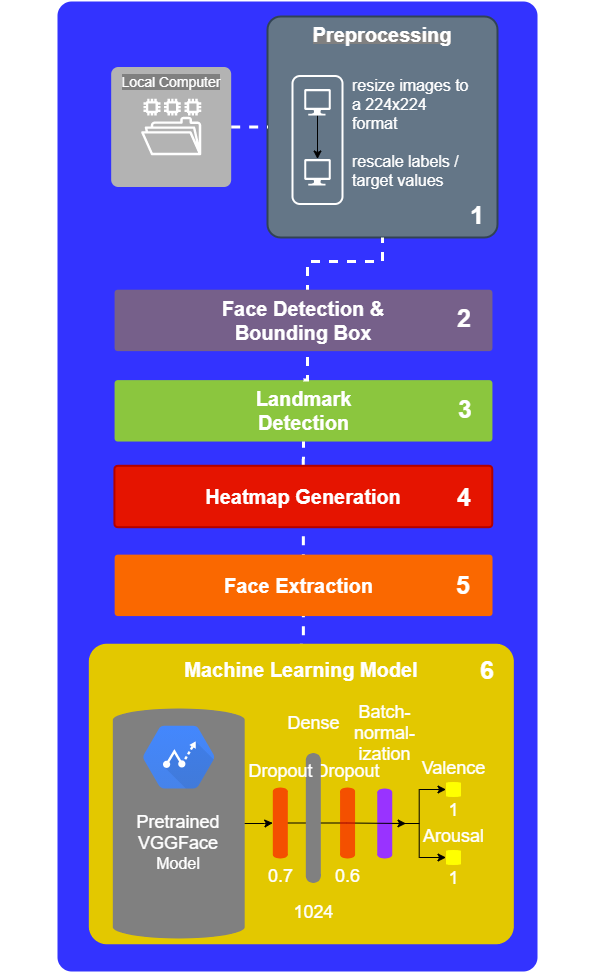
\includegraphics[width=0.55\textwidth]{Figures/DataFlow_Diagram_new.png}}
  \caption{Emotion recognition pipeline in this Master's thesis requires seven essential steps.}
  \label{fig:MachineLearningModelMethods}
  \end{center}
\end{figure}

Figure \ref{fig:MachineLearningModelMethods} illustrates the emotion recognition pipeline in this Master's thesis that consists of six essential steps. First, video frames were resized to a 224x224 format, and data was being standardized by subtracting the training data mean. Second, the face was detected and a bounding box was determined using a pre-trained network optimized for face detection, namely MTCNN \citep{Zhang:2016:MTCCN}. Third, landmarks were detected based on the previously determined bounding box. 
\newline\newline
Fourth, a heatmap was generated using the detected landmarks which was subsequently applied as an overlay to the original image. Fifth, the face was extracted from the image by cropping it along the borders of the bounding box. Sixth, data augmentation was applied in order to significantly increase the diversity of the images in the underlying dataset. Seventh, data was passed into the machine learning model, consisting of a the pre-trained VGGFace neural network that was extended with a custom classifier.

%%%%%%%%%%%%%%%%%%%%%%%
\section{Preprocessing}
The very first step in the pipeline shown in figure \ref{fig:MachineLearningModelMethods} is the preprocessing of both, the input images, as well as the output labels. Input images were resized to the size of 224x224 pixels, as is also required by the pre-trained neural network VGGFace \citep{Cao:2018:VGGFace2}. Output labels, originally in the scale of -10 to +10, were re-scaled to -1 to +1 in order to fit the chosen 'tanh' activation function.
\newline\newline
Samples of the resized input images and their corresponding output labels are shown in figure \ref{fig:MethodologyPreprocess}. Output labels consist of valence (=expression of how positive or negative an emotion is) and arousal (=expression of how strong or weak an emotion is).

\begin{figure}[H]
  \centering
  \subfloat[V: 0.0, A: +0.5]{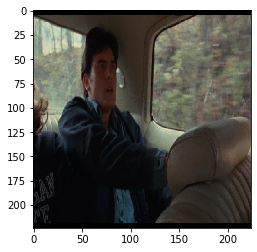
\includegraphics[width=0.33\textwidth]{Figures/preprocessing/001_00000.png}}
  \hfill
  \subfloat[V: +0.2, A: +0.3]{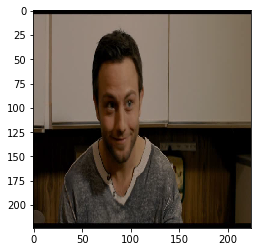
\includegraphics[width=0.33\textwidth]{Figures/preprocessing/002_00000.png}}
  \hfill
  \subfloat[V: -0.5, A: +0.3]{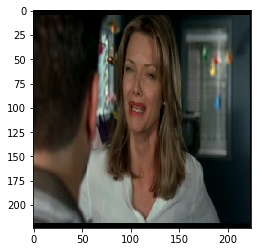
\includegraphics[width=0.33\textwidth]{Figures/preprocessing/576_00000.png}}
  
  \subfloat[V: 0.0, A: +0.5]{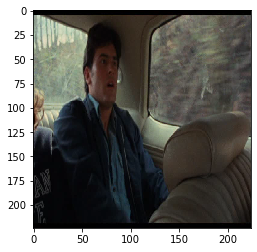
\includegraphics[width=0.33\textwidth]{Figures/preprocessing/001_00011.png}}
  \hfill
  \subfloat[V: +0.2, A: +0.4]{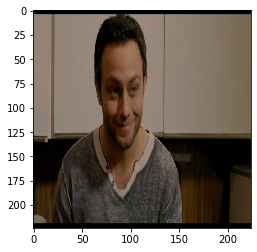
\includegraphics[width=0.33\textwidth]{Figures/preprocessing/002_00011.png}}
  \hfill
  \subfloat[V: -0.6, A: +0.3]{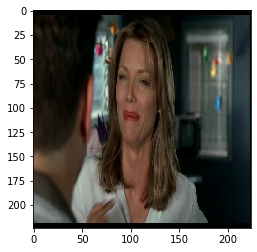
\includegraphics[width=0.33\textwidth]{Figures/preprocessing/576_00011.png}}
  \caption{Preprocessed sample frames from the AFEW-VA dataset \citep{Kossaifi:2017:AFEW-VADatabase} and their corresponding labels representing the valence (V) and arousal (A) as values between -1 and +1.}
  \label{fig:MethodologyPreprocess}
\end{figure}


\section{Face Detection}
The second step in the proposed pipeline involves detecting the faces in each frame of the video. This is valuable in order to determine the face's bounding box which is need in a further stage of the pipeline for the detection of landmarks and the cropping of the image. To achieve this, the Multi-Task Cascaded Convolutional Neural Network (MTCNN) by \citet{Zhang:2016:MTCCN} was used.
\newline\newline
MTCNN is a pre-trained neural network optimized for the tasks of simultaneous face detection, face alignment, bounding boxing and landmark detection \citep{Brownlee:2019:VggFace2HowToFaceRec}. This makes it ideal for the purpose of determining the face's bounding box in the face of the video frames. In figure \ref{fig:MethodologyBoundingBox} successful examples of the application of the MTCNN algorithm are shown by overlaying the bounding box on the image.

\begin{figure}[H]
  \centering
  \subfloat[V: 0.0, A: +0.5]{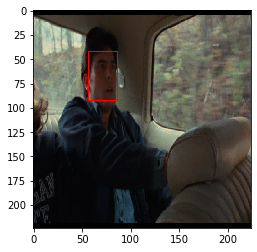
\includegraphics[width=0.33\textwidth]{Figures/boundingbox/001_00000.png}}
  \hfill
  \subfloat[V: +0.2, A: +0.3]{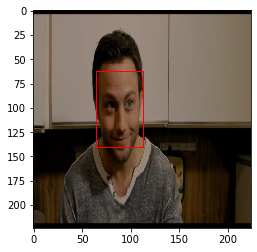
\includegraphics[width=0.33\textwidth]{Figures/boundingbox/002_00000.png}}
  \hfill
  \subfloat[V: -0.5, A: +0.3]{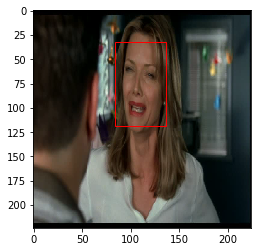
\includegraphics[width=0.33\textwidth]{Figures/boundingbox/576_00000.png}}
  
  \subfloat[V: 0.0, A: +0.5]{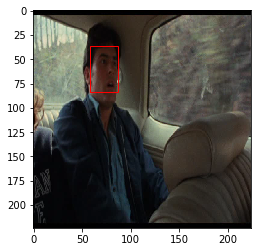
\includegraphics[width=0.33\textwidth]{Figures/boundingbox/001_00011.png}}
  \hfill
  \subfloat[V: +0.2, A: +0.4]{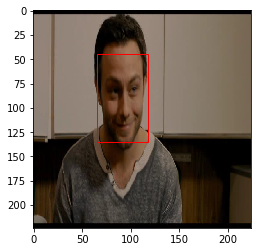
\includegraphics[width=0.33\textwidth]{Figures/boundingbox/002_00011.png}}
  \hfill
  \subfloat[V: -0.6, A: +0.3]{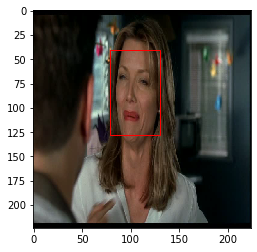
\includegraphics[width=0.33\textwidth]{Figures/boundingbox/576_00011.png}}
  \caption{Visualization of the bounding box detected by the MTCNN face detection module \citep{Zhang:2016:MTCCN} and their corresponding labels representing the valence (V) and arousal (A) as values between -1 and +1.}
  \label{fig:MethodologyBoundingBox}
\end{figure}



\section{Landmark Detection}
The third step in the proposed pipeline involves the detection of facial landmarks in each frame. This is a preliminary step for the generation of the heatmap, as it is based on the coordinates of the landmark points.
\newline\newline
This was done using a 'Face Landmark Detection' algorithm based on the work done by \citet{Kazemi:2014:ShapePredictor}. The algorithm is based on an ensemble of regression trees which successively aligns the constructed shape model to the specific features of the the face at hand.
\newline\newline
The input of the algorithm consists of the frame, as well as coordinates of the face's bounding box. The algorithm's output is made up of 68 facial landmarks of a person's face. Examples of this successful operation are shown in figure \ref{fig:MethodologyLandmarks} by overlaying the landmark dots on the input image.
\citep{Datahacker:2020:DlibFacialLandmarks}

\begin{figure}[H]
  \centering
  \subfloat[V: 0.0, A: +0.5]{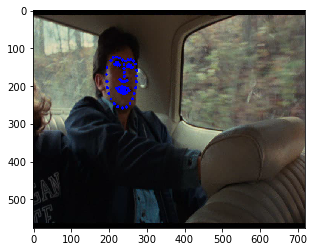
\includegraphics[width=0.33\textwidth]{Figures/landmarks/001_00000.png}}
  \hfill
  \subfloat[V: +0.2, A: +0.3]{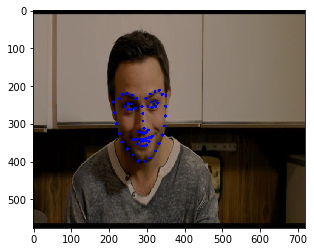
\includegraphics[width=0.33\textwidth]{Figures/landmarks/002_00000.png}}
  \hfill
  \subfloat[V: -0.5, A: +0.3]{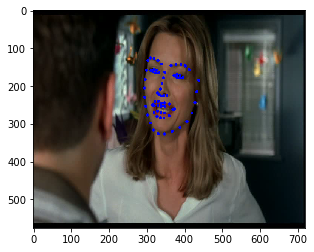
\includegraphics[width=0.33\textwidth]{Figures/landmarks/576_00000.png}}
  
  \subfloat[V: 0.0, A: +0.5]{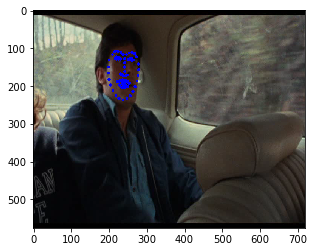
\includegraphics[width=0.33\textwidth]{Figures/landmarks/001_00011.png}}
  \hfill
  \subfloat[V: +0.2, A: +0.4]{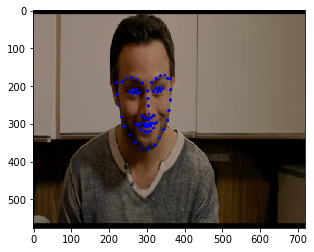
\includegraphics[width=0.33\textwidth]{Figures/landmarks/002_00011.png}}
  \hfill
  \subfloat[V: -0.6, A: +0.3]{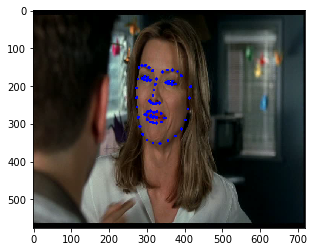
\includegraphics[width=0.33\textwidth]{Figures/landmarks/576_00011.png}}
  \caption{Visualization of the landmarks detected by the pre-trained 'Face Landmark Detection' algorithm \citep{Kazemi:2014:ShapePredictor} and their corresponding labels representing the valence (V) and arousal (A) as values between -1 and +1.}
  \label{fig:MethodologyLandmarks}
\end{figure}


%%%%%%%%%%%%%%%%%%%%%%%%%%%%%%%%%%%%%%%%%%%%%%%%%%%%%
\section{Heatmap Generation}
The fourth step of this work's pipeline involves the conversion of landmarks into a heatmap overlay. This is valuable so that the neural network can learn to differentiate between how important an area is. This was done using an augmentation technique proposed by \citet[~para. 1]{Jung:2020:Imgaug}. Results of this conversion can be seen in the figure \ref{fig:MethodologyHeatmap}.

\begin{figure}[H]
  \centering
  \subfloat[V: 0.0, A: +0.5]{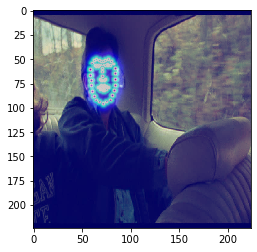
\includegraphics[width=0.33\textwidth]{Figures/heatmap/001_00000.png}}
  \hfill
  \subfloat[V: +0.2, A: +0.3]{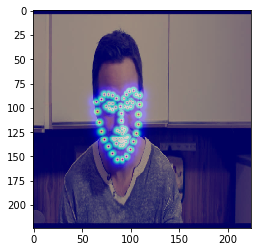
\includegraphics[width=0.33\textwidth]{Figures/heatmap/002_00000.png}}
  \hfill
  \subfloat[V: -0.5, A: +0.3]{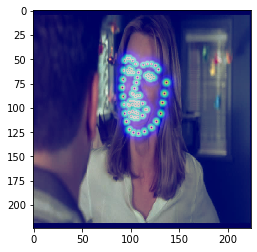
\includegraphics[width=0.33\textwidth]{Figures/heatmap/576_00000.png}}
  
  \subfloat[V: 0.0, A: +0.5]{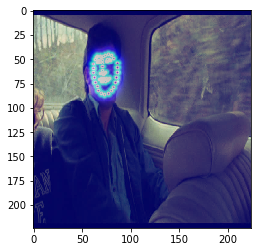
\includegraphics[width=0.33\textwidth]{Figures/heatmap/001_00011.png}}
  \hfill
  \subfloat[V: +0.2, A: +0.4]{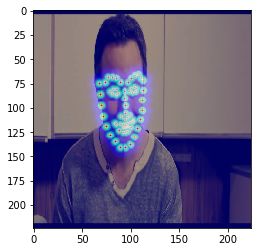
\includegraphics[width=0.33\textwidth]{Figures/heatmap/002_00011.png}}
  \hfill
  \subfloat[V: -0.6, A: +0.3]{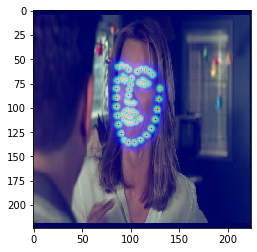
\includegraphics[width=0.33\textwidth]{Figures/heatmap/576_00011.png}}
  \caption{Visualization of the heatmap generated by imgaug algorithm \citep{Jung:2020:Imgaug} and their corresponding labels representing the valence (V) and arousal (A) as values between -1 and +1.}
  \label{fig:MethodologyHeatmap}
\end{figure}


%%%%%%%%%%%%%%%%%%%%%%%%%%%%%%%%%%%%%%%%%%%%%%%%%%%%%
\section{Face Extraction}
The fifth step in the proposed pipeline involves the extraction of the face from the original input image. This is valuable as it removes unimportant information/features of the image's background which could otherwise negatively affect the learning process.
\newline\newline
This step was conducted by simply cropping the face along the border lines of the face's bounding box. The output is again a image with a dimensions of 224x224 pixels that displays the inner area of the bounding box, namely the person's face. Example outputs are illustrated in figure \ref{fig:MethodologyExtraction}.

\begin{figure}[H]
  \centering
  \subfloat[V: 0.0, A: +0.5]{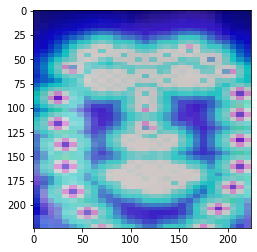
\includegraphics[width=0.33\textwidth]{Figures/extraction/001_00000.png}}
  \hfill
  \subfloat[V: +0.2, A: +0.3]{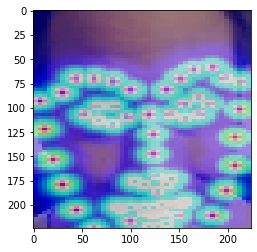
\includegraphics[width=0.33\textwidth]{Figures/extraction/002_00000.png}}
  \hfill
  \subfloat[V: -0.5, A: +0.3]{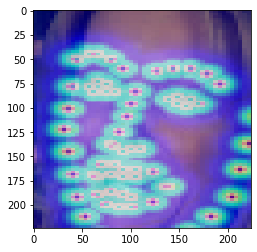
\includegraphics[width=0.33\textwidth]{Figures/extraction/576_00000.png}}
  
  \subfloat[V: 0.0, A: +0.5]{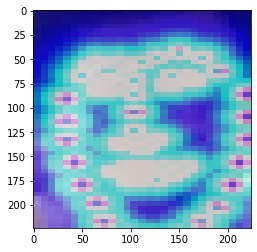
\includegraphics[width=0.33\textwidth]{Figures/extraction/001_00011.png}}
  \hfill
  \subfloat[V: +0.2, A: +0.4]{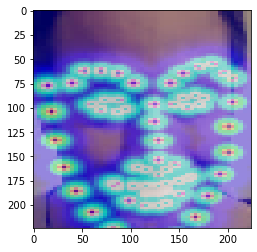
\includegraphics[width=0.33\textwidth]{Figures/extraction/002_00011.png}}
  \hfill
  \subfloat[V: -0.6, A: +0.3]{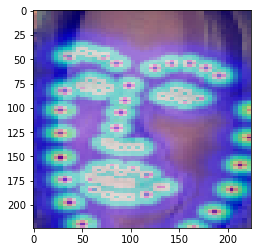
\includegraphics[width=0.33\textwidth]{Figures/extraction/576_00011.png}}
  \caption{Visualization of the extracted face showing the previously applied heatmap, and their corresponding labels representing the valence (V) and arousal (A) as values between -1 and +1.}
  \label{fig:MethodologyExtraction}
\end{figure}


%%%%%%%%%%%%%%%%%%%%%%%%%%%%%%%%%%%%%%%%%%%%%%%%%%%%%
\section{Machine Learning Model for Emotion Recognition}
In the final step of the proposed pipeline, the cropped frames are fed into the machine learning model for training on the emotion recognition challenge. The model's architecture, consisting of the pre-trained VGGFace model \citep{Cao:2018:VGGFace2} and a custom classifier, can be seen in figure \ref{fig:MachineLearningModel}.
\newline\newline
The VGGFace model architecture, is based on the famous ResNet-50 convolutional neural network which the authors \citet{Cao:2018:VGGFace2} pre-trained on a large-scale face dataset, named VGGFace2. The dataset contains about 3.31 million images of 9131 subjects and poses, which provided a wide variety of poses, ages, etc. When the VGGFace2 paper, written by \citet{Cao:2018:VGGFace2}, was published in \citeyear{Cao:2018:VGGFace2}, it exceeded the performance of previous state-of-the-art by a large margin \citep{Cao:2018:VGGFace2}.

\begin{figure}[H]
  \begin{center}
  \makebox[\textwidth][c]{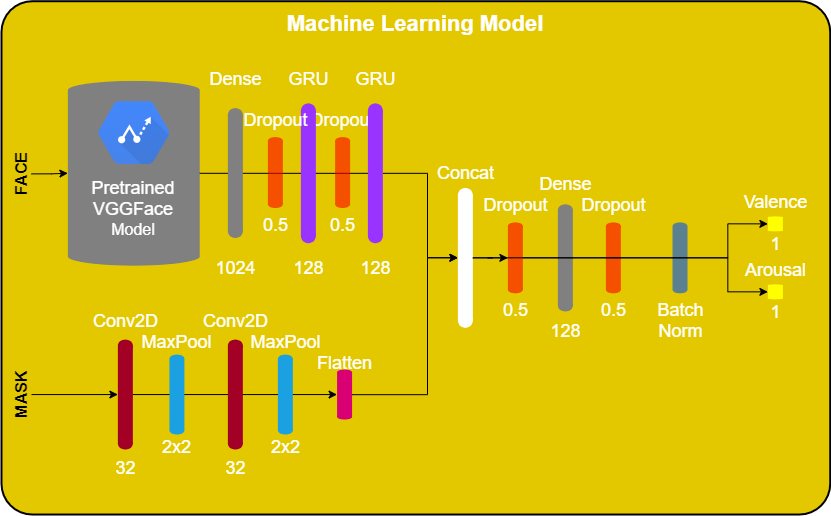
\includegraphics[width=0.6\textwidth]{Figures/MachineLearningModel.png}}
  \caption{The machine learning model consists of the pre-trained VGGFace network where the last layers were replaced by a custom classifier.}
  \label{fig:MachineLearningModel}
  \end{center}
\end{figure}

The utilization of a pre-trained neural network is often referred to as transfer learning. \citet{Pedro:2018:TransferLearning} supports that instead of training the model from scratch, transfer learning allows to start the training process from patterns that have already been learned by solving a different problem.
\newline\newline
In this work, a version of the VGGFace model that was pre-trained on the VGGFace2 dataset \citep{Cao:2018:VGGFace2} for the task of face identification has been used. The pre-trained model was then further fine-tuned on the AFEW-VA dataset \citep{Kossaifi:2017:AFEW-VADatabase}. In this way, learnt patterns about facial features from the face identification task were used to kick-start the learning for emotion recognition from there. 
\newline\newline
A noteworthy architectural change was the removal of the last fully-connected layers at the end of VGGFace. For this work, these layers were replaced with another classifier in order to learn the correlation between facial features and their target labels for the emotion recognition task. The architecture of the newly added classifier is shown in figure \ref{fig:MachineLearningModel}.